\documentclass[journal,12pt,twocolumn]{IEEEtran}
\usepackage{amsmath,amssymb,amsfonts,amsthm}
\usepackage{txfonts}
\usepackage{tkz-euclide}
\usepackage{listings}
\usepackage{gvv}
\usepackage[latin1]{inputenc}
\usepackage{array}
\usepackage{pgf}
\usepackage{lmodern}

\begin{document}
\bibliographystyle{IEEEtran}

\vspace{3cm}

\title{}
\author{EE23BTECH11024 - G.Karthik Yadav$^{*}$
}
\maketitle
\newpage
\bigskip



\section*{11.9.5.14}
\noindent 1. \hspace{2pt}Let S be the sum, P the product and R the sum of reciprocals of n terms in a G.P.
Prove that $P^2 R^n = S^n$.\\

\solution

from table \ref{tab:24.11.9.5.14}
\setlength{\arrayrulewidth}{0.2mm}
\setlength{\tabcolsep}{15pt}
\renewcommand{\arraystretch}{1.15}


\begin{table}[ht]
  \centering
  \begin{tabular}{|c|c|c|}
    \hline
    	Symbol & Parameters & value\\
    \hline
	  $u\brak{n}$ & unit step function & 1, if n$\geq$ 0; \\& &0 otherwise \\
    \hline
	  $r$ & common ratio of GP &  \\	  
    \hline
	  $x\brak{n}$ & general term in a GP & $x\brak{0} r^{n}$ \\
    \hline
	  $y\brak{n}$ & general term of reciprocal terms in a GP & $\frac{r^{-n}}{x\brak{0}}$ \\
	 	 
    \hline
  \end{tabular}
  \vspace{0.3cm}
  \caption{Input Parameters}
  \label{tab:24.11.9.5.14}
\end{table}

\begin{align}
    x \brak{n} & = x\brak{0}r^{n}  
\end{align}    
Using \eqref{11024_gp_sum},
\begin{align}
    S = x\brak{0}\brak{\frac{r^{n+1}-1}{r-1}}u\brak{n} \label{24.11.9.5.14.1}
\end{align}

\begin{align}
    y\brak{n} &= \frac{1}{x\brak{0}} r^{-n}
\end{align}

Using \eqref{11024_gp_sum} and setting the first term as $\frac{1}{x\brak{0}}$ and common ratio as $r^{-1}$,
\begin{align}
    R = \frac{1}{x\brak{0}}\brak{\frac{1-r^{-\brak{n+1}}}{1-r^{-1}}} \label{24.11.9.5.14.2}
\end{align}

\begin{align}
    P = \brak{x\brak{0}}^{n+1} r^{n(n+1)} \label{24.11.9.5.14.3}
\end{align}
by using eq \eqref{24.11.9.5.14.1}, eq \eqref{24.11.9.5.14.2} and eq \eqref{24.11.9.5.14.3} \\
$P^2 R^n = S^n$.

\begin{figure}[ht]
   \centering
   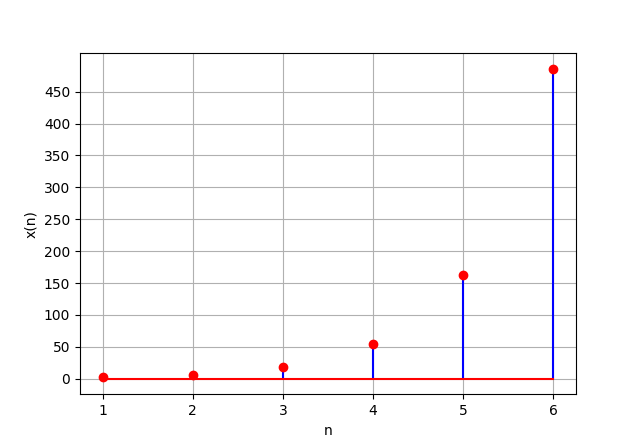
\includegraphics[width=1\columnwidth]{figs/plot2.png}
   \caption{Stem Plot of $x\brak{n} = \brak{2}3^{n} , x\brak{0} = 2$ and $r = 3$}
   \label{fig: 1.11.9.1.1}
\end{figure}

\begin{figure}[ht]
   \centering
   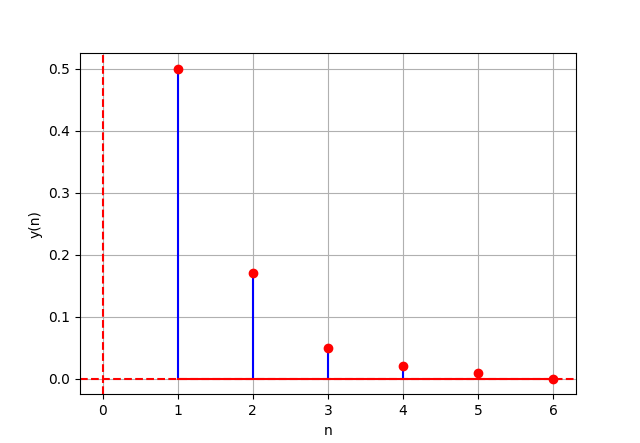
\includegraphics[width=1\columnwidth]{figs/plot3.png}
   \caption{Stem Plot of $y\brak{n} = \brak{0.5}3^{-n} , x\brak{0} = 2$ and $r = 3$}
   \label{fig: 1.11.9.1.1}
\end{figure}


\end{document}
